\section{Topic Tree}
\subsection{Overview}
Most learning management systems do not have a simple and easy method to import course material and resources from other courses. Some LMS platforms such as OpenLearning have no method of importing any data at all, and other platforms such as Canvas allows you to import crowd sourced material into your own course, however still does not allow you to import topics of resources. \\

This new LMS has a new topic tree feature, which will allow teachers and academics to add course material under a specific topic instead.\\

\textbf{Topics} \\
A topic is a collection of educational material that is related to a particular subject. For example, in UNSW's Introduction to Programming course (COMP1511), one of the topics in the course is ``Pointers", which contains all course material related to pointers.\\

At Charles Sturt University, each topic is defined as a small subject that is three hours in length \cite{csutopictree}. CSU's curriculum covers around 1000 topics with each topic being three hours in length for a degree. In this thesis, we will also define a topic being three hours of content, but instructors can choose what amount of content constitutes as a topic.\\

\textbf{Topic Groups} \\
Topic groups are similar to courses themselves, except they are purely for organisational and enrolment purposes. We found that it would be much easier to enrol students into a group of topics instead of each individual topic, and it makes searching the topic tree much easier as there are a smaller number of topic groups than topics themselves. \\

Topic groups themselves do not contain assessments, exams, or any other resources. Only topics themselves contain this information. Therefore, academics must store assessments in individual topics and set up the prerequisites so if they wish, they can store a final exam in the last topic that students must complete or in an empty "milestone" topic. We decided to name this grouping of topics as "topic groups" instead of courses due to how a traditional course contains assessments and other content for the entire course, and does not have prerequisites between the topics themselves. This naming helps differentiate the system from the traditional university model.\\

\textbf{Prerequisites} \\

Each topic can have its own prerequisites, as discussed briefly previously. Some topics must be completed in order to complete the current topic. Prerequisites can be across topic groups as well. For example, Linked Lists in the "Introduction to Programming" topic group must be completed in order to start Graphs in "Data Structures and Algorithms". This improves reusability, as topics in other topic groups can be set as prerequisites eg. Git can be set a prerequisite for "Web Front end Programming" instead.

\textbf{Reusability} \\
The topic tree enables academics to easily reuse content - by setting specific topics, academics can reuse content instead of creating new content for the same topic in their own course. A good example of this is "Web Front end Programming" at UNSW - Instead of creating new content for Git, academics can set Git as a prerequisite. However, to encourage reusability, a cloning feature is also provided where academics can clone a topic and its resources from another topic group and put it in its own topic group. This further enables reusability, demonstrating that there is no need to spend time creating new content.\\

\textbf{Course Materials} \\
The Meta Learning Management System also organises content into four sections:
\begin{itemize}
    \item Content
    \item Practice
    \item Preparation
    \item Assessments
\end{itemize}

These various sections were chosen as they fit many learning models, including UNSW's learning models as listed on their website \cite{learningModel}. Students are introduced to it in the content section, and then get to know more about it in the practice section, and try it out in the preparation and assessments sections. After receiving feedback, this cycle repeats again.\\

\begin{figure}[h!]
    \centering
    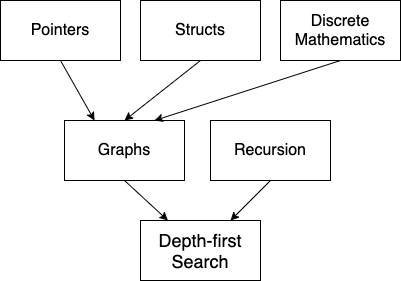
\includegraphics[scale=0.4]{topic-tree-example}
    \caption{Example of a topic tree with Depth first search}
\end{figure}

In the above example, pointers, structs and discrete mathematics must be learned in order to learn graphs. Likewise, graphs and recursion is required to learn depth first search.\\

\subsection{Initial Designs}
\begin{figure}[h!]
    \centering
    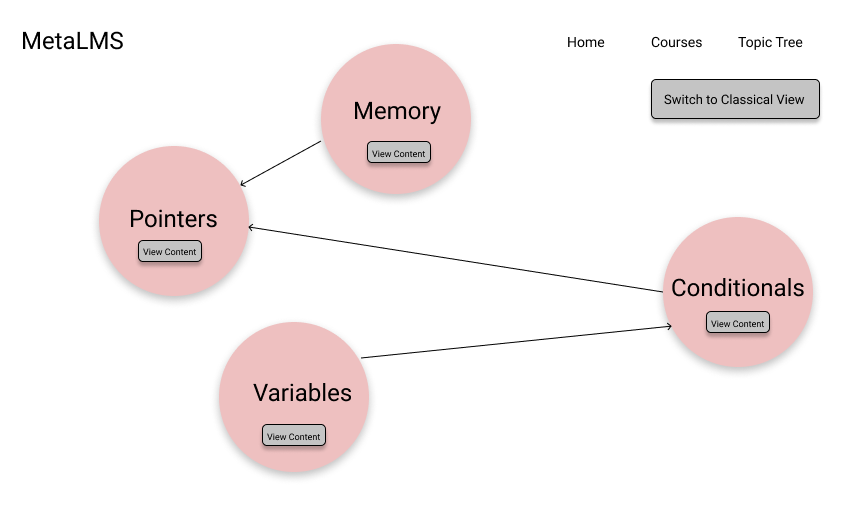
\includegraphics[scale=0.4]{topic-tree-graph-view}
    \caption{Topic Groups Graph UI}
\end{figure}

The above design is an initial design of the graph view of the topic tree. It was intended that there would only be topics when the topic tree was first designed, and the user could select a topic group to view the topic tree for that topic group. However, it was impossible to view prerequisites across topic groups with this design, and made it more difficult to view topics inside different topic groups. Therefore, a new design was chosen as follows.

\begin{figure}[h!]
    \centering
    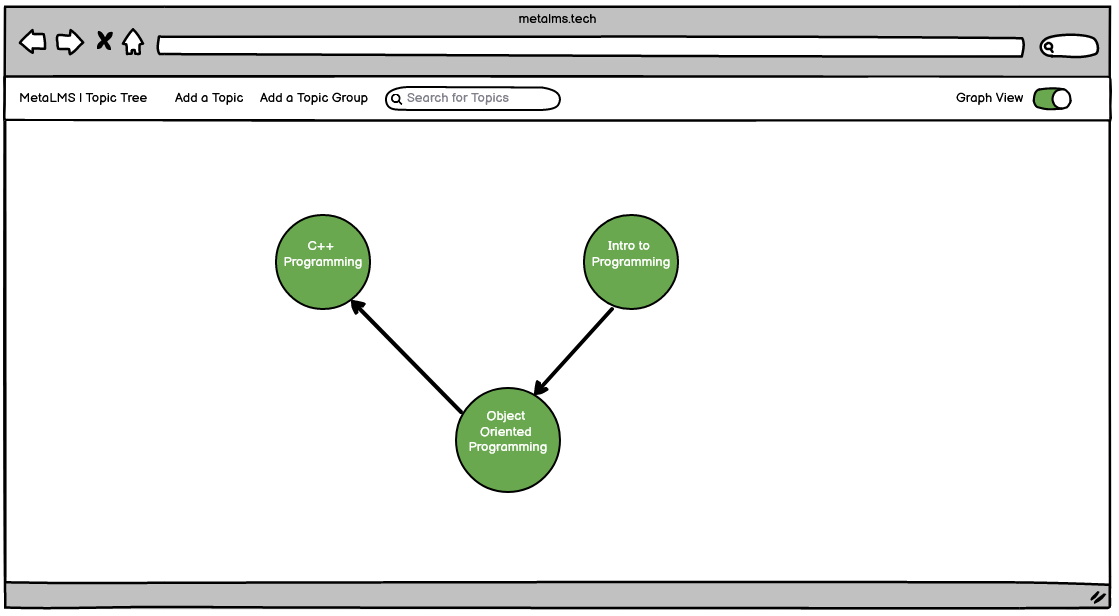
\includegraphics[scale=0.4]{topic-tree-graph-view-final-design}
    \caption{Topic Groups Graph UI Final Design}
\end{figure}

Instead, the topic groups are all shown on one graph, and a simple toggle to switch between the list view and the graph view is displayed in the top right. There are more options to add topic groups or topics at the top, and the user can click a topic group to show the individual topics as shown below.


\begin{figure}[h!]
    \centering
    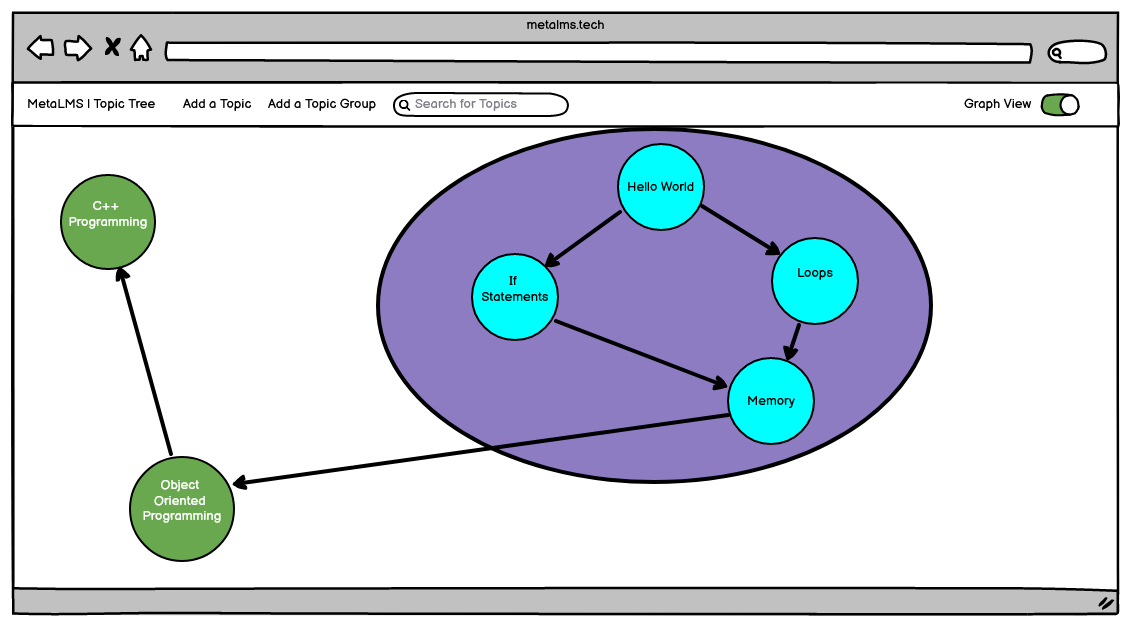
\includegraphics[scale=0.4]{topic-tree-expanded-design}
    \caption{Topic Groups Graph UI Expanded Topics}
\end{figure}

As shown, when a topic group is clicked, a hull in the background surrounds the topics to indicate they are part of the same group. Topics are shown in blue, and the individual prerequisites are shown with prerequisites pointing to topics in other topic groups as well. 

\begin{figure}[h!]
    \centering
    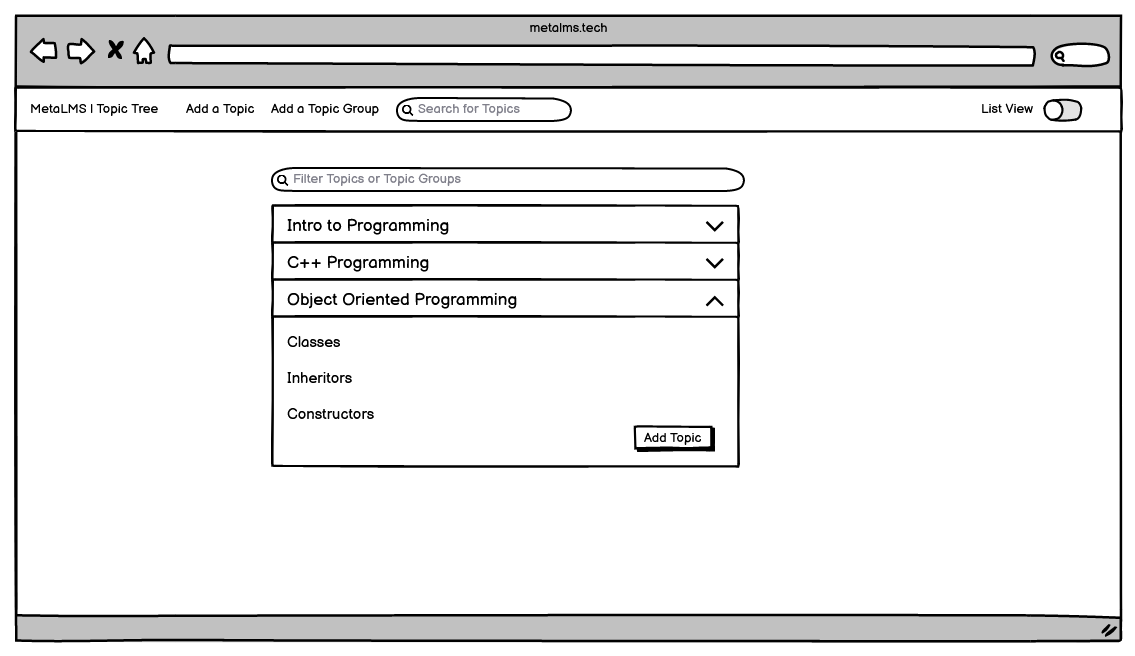
\includegraphics[scale=0.4]{topic-tree-list-view-final-design}
    \caption{Topic Groups List UI Final Design}
\end{figure}

The final design of the list view shows both topics and topic groups on the same page to improve performance and usability, as there is less of a need to click through different pages to view different topic groups. Users can click on a specific topic group to expand and show the topics inside it, and click Add Topic to add a specific topic. Topics can be clicked to view their prerequisites.

\subsection{Requirements}
Each requirement will have a priority: High, Medium or Low. High priority requirements will be completed first, and then medium and low priority requirements respectively. \\

\subsection{Functional Requirements}

\textbf{Viewing Topics}
\FloatBarrier
\begin{table}[h!]
\begin{tabular}{|l|l|}
\hline
\textit{As a}      & User                                                \\ \hline
\textit{I want to} & View groups of topics                               \\ \hline
\textit{So that}   & I can see how topic groups interact with each other \\ \hline
\textit{Priority}  & {\color[HTML]{FE996B} Medium}                         \\ \hline
\textit{Status}    & Complete                                            \\ \hline
\end{tabular}
\end{table}


\begin{table}[h!]
\begin{tabular}{|l|l|}
\hline
\textit{As a}      & User                                                \\ \hline
\textit{I want to} & View topics within each topic group                 \\ \hline
\textit{So that}   & I can see how topic groups interact with each other \\ \hline
\textit{Priority}  & {\color[HTML]{FE0000} High}                         \\ \hline
\textit{Status}    & Complete                                            \\ \hline
\end{tabular}
\end{table}

\begin{table}[h!]
\begin{tabular}{|l|l|}
\hline
\textit{As a}      & User                                                \\ \hline
\textit{I want to} & View topics within each topic group                 \\ \hline
\textit{So that}   & I can see how topic groups interact with each other \\ \hline
\textit{Priority}  & {\color[HTML]{FE0000} High}                         \\ \hline
\textit{Status}    & Complete                                            \\ \hline
\end{tabular}
\end{table}

\begin{table}[h!]
\begin{tabular}{|l|l|}
\hline
\textit{As a}      & User                                                           \\ \hline
\textit{I want to} & Search for specific resources                                  \\ \hline
\textit{So that}   & I can find other resources easily in the many topics available \\ \hline
\textit{Priority}  & {\color[HTML]{FE0000} High}                                    \\ \hline
\textit{Status}    & Not Complete                                                   \\ \hline          
\end{tabular}
\end{table}

\begin{table}[h!]
\begin{tabular}{|l|l|}
\hline
\textit{As a}      & User                                                                            \\ \hline
\textit{I want to} & View topic prerequisites                                                        \\ \hline
\textit{So that}   & I can see which topics must be completed in order to complete the current topic \\ \hline
\textit{Priority}  & {\color[HTML]{FE996B} Medium}                                                     \\ \hline
\textit{Status}    & Complete                                                                        \\ \hline                              
\end{tabular}
\end{table}

\begin{table}[h!]
\begin{tabular}{|l|l|}
\hline
\textit{As a}      & User                                                   \\ \hline
\textit{I want to} & view a graph of topics and their prerequisites         \\ \hline
\textit{So that}   & The topics and their prerequisites are easily viewable \\ \hline
\textit{Priority}  & {\color[HTML]{FE0000} High}                            \\ \hline
\textit{Status}    & Complete                                               \\ \hline      
\end{tabular}
\end{table}

\begin{table}[h!]
\begin{tabular}{|l|l|}
\hline
\textit{As a}      & User                                                              \\ \hline
\textit{I want to} & view the topic tree with a traditional interface                  \\ \hline
\textit{So that}   & topics can be viewed more easily using a less confusing interface \\ \hline
\textit{Priority}  & {\color[HTML]{3166FF} Low}                                        \\ \hline
\textit{Status}    & Complete                                                          \\ \hline
\end{tabular}
\end{table}
\FloatBarrier

\textbf{Adding Topics and resources}
\FloatBarrier
\begin{table}[h!]
\begin{tabular}{|l|l|}
\hline
\textit{As a}      & User                                           \\ \hline
\textit{I want to} & add a new topic                                \\ \hline
\textit{So that}   & I can edit the topic tree and add more content \\ \hline
\textit{Priority}  & {\color[HTML]{FE0000} High}                    \\ \hline
\textit{Status}    & Complete                                       \\ \hline              
\end{tabular}
\end{table}

\begin{table}[h!]
\begin{tabular}{|l|l|}
\hline
\textit{As a}      & Academic                       \\ \hline
\textit{I want to} & upload course material      \\ \hline
\textit{So that}   & I can add content to topics       \\ \hline
\textit{Priority}  & {\color[HTML]{FE0000} High} \\ \hline
\textit{Status}    & Complete                    \\ \hline 
\end{tabular}
\end{table}

\begin{table}[h!]
\begin{tabular}{|l|l|}
\hline
\textit{As a}      & Academic                                                                      \\ \hline
\textit{I want to} & add a new topic group                                                     \\ \hline
\textit{So that}   & topics are more organised and I can create new topics under the new group \\ \hline
\textit{Priority}  & {\color[HTML]{F8A102} Medium}                                             \\ \hline
\textit{Status}    & Complete                                                                  \\ \hline
\end{tabular}
\end{table}

\begin{table}[h!]
\begin{tabular}{|l|l|}
\hline
\textit{As a}      & Academic                                 \\ \hline
\textit{I want to} & Add tags to a topic                      \\ \hline
\textit{So that}   & Search for topics faster and more easily \\ \hline
\textit{Priority}  & {\color[HTML]{3531FF} Low}               \\ \hline
\textit{Status}    & Complete                                 \\ \hline
\end{tabular}
\end{table}

\begin{table}[h!]
\begin{tabular}{|l|l|}
\hline
\textit{As a}      & Academic                                                                      \\ \hline
\textit{I want to} & add a new topic group                                                     \\ \hline
\textit{So that}   & topics are more organised and I can create new topics under the new group \\ \hline
\textit{Priority}  & {\color[HTML]{F8A102} Medium}                                             \\ \hline
\textit{Status}    & Complete                                                                  \\ \hline
\end{tabular}
\end{table}
\FloatBarrier
\textbf{Deleting Topics}
\FloatBarrier
\begin{table}[h!]
\begin{tabular}{|l|l|}
\hline
\textit{As a}      & Academic                                 \\ \hline
\textit{I want to} & delete a topic that I've created         \\ \hline
\textit{So that}   & I can remove content from the topic tree \\ \hline
\textit{Priority}  & {\color[HTML]{FE0000} High}              \\ \hline
\textit{Status}    & Complete                                 \\ \hline
\end{tabular}
\end{table}

\begin{table}[h!]
\begin{tabular}{|l|l|}
\hline
\textit{As a}      & Academic                                 \\ \hline
\textit{I want to} & delete a topic group that I've created   \\ \hline
\textit{So that}   & I can remove content from the topic tree \\ \hline
\textit{Priority}  & {\color[HTML]{F8A102} Medium}              \\ \hline
\textit{Status}    & Not Complete                                 \\ \hline
\end{tabular}
\end{table}

\begin{table}[h!]
\begin{tabular}{|l|l|}
\hline
\textit{As a}      & Academic                                                    \\ \hline
\textit{I want to} & remove course material from a topic                         \\ \hline
\textit{So that}   & I can remove content from the topic tree that is not needed \\ \hline
\textit{Priority}  & {\color[HTML]{FE0000} High}                                 \\ \hline
\textit{Status}    & Complete                                                    \\ \hline
\end{tabular}
\end{table}
\FloatBarrier
\textbf{Topic Prequisites}
\FloatBarrier
\begin{table}[h!]
\begin{tabular}{|l|l|}
\hline
\textit{As a}      & Academic                                                                               \\ \hline
\textit{I want to} & add a topic prerequisite                                                               \\ \hline
\textit{So that}   & I can require other topics to be completed before students can learn the current topic \\ \hline
\textit{Priority}  & {\color[HTML]{FE996B} Medium}                                                            \\ \hline
\textit{Status}    & Complete                                                                               \\ \hline
\end{tabular}
\end{table}

\begin{table}[h!]
\begin{tabular}{|l|l|}
\hline
\textit{As a}      & Academic                                                                               \\ \hline
\textit{I want to} & delete a topic prerequisite                                                            \\ \hline
\textit{So that}   & I can remove requirements for a topic \\ \hline
\textit{Priority}  & {\color[HTML]{FE996B} Medium}                                                          \\ \hline
\textit{Status}    & Complete                                                                               \\ \hline
\end{tabular}
\end{table}
\FloatBarrier
\textbf{Integration}
\FloatBarrier
\begin{table}[h!]
\begin{tabular}{|l|l|}
\hline
\textit{As a}      & Academic                                                  \\ \hline
\textit{I want to} & allow third party integration such as YouTube and The Box \\ \hline
\textit{So that}   & I can use external services with the topic tree           \\ \hline
\textit{Priority}  & {\color[HTML]{3531FF} Low}                                \\ \hline
\textit{Status}    & Not Complete                                              \\ \hline
\end{tabular}
\end{table}
\FloatBarrier
\textbf{Exporting}
\FloatBarrier
\begin{table}[h!]
\begin{tabular}{|l|l|}
\hline
\textit{As a}      & Academic                                          \\ \hline
\textit{I want to} & Export data from topics and course material       \\ \hline
\textit{So that}   & I can use the topic tree data with other services \\ \hline
\textit{Priority}  & {\color[HTML]{3531FF} Low}                        \\ \hline
\textit{Status}    & Not Complete                                      \\ \hline
\end{tabular}
\end{table}
\FloatBarrier
\subsection{Non Functional requirements}
The feature also has non functional requirements in order to better evaluate the completion of the feature. \\

\textbf{Performance} \\
Performance must be high and the feature must be responsive to provide a high quality user experience for both academics and students. Performance will be assessed using tools such as Google Lighthouse \cite{googleLighthouse}. Google Lighthouse uses several metrics to assess performance, as explained previously. \\

\textbf{Accessibility} \\
The topic tree feature will also be assessed on how accessible the interface is. If features such as alt tags, high contrast colours and keyboard navigation are not implemented then not all academics and students will be able to use the topic tree feature. Therefore, tools such as Google Lighthouse will be used to access its accessibility as the tool also includes metrics for measuring accessibility of a website \cite{googleLighthouseAccessibility}. \\

\textbf{Usability} \\
Finally, the feature will be assessed on its usability. This includes whether the topic tree feature is attractive and easy to use. Various students and academics will be surveyed on how easy they found the system to use. The number of errors and time taken to complete a task will also be assessed.\\

\subsection {Changes from inital requirements}

The initial requirements did not mention anything about third party integration such as integrating YouTube and The Box. Later, it was realised that third party services would be very useful in uploading files and managing content, and so the requirement was added.\\

Originally, the requirements also stated that there should be functionality to upload course material by selecting multiple topics. This did not make sense in the context of the topic tree, as course material is attached to specific topics, not topic groups, and so was removed from the final requirements.\\

Finally, tags were added to the final requirements. The searchability of the topic tree proved a difficult problem to solve, and by adding tags to topics, users would be able to search specific topics by their tags instead of by name. This was then added to the list of requirements as it greatly improved the searchability of the topic tree.\\